\documentclass{article}
\usepackage{amsmath}
\usepackage{bbm}
\usepackage{amssymb}
\usepackage[ruled,vlined]{algorithm2e}
\usepackage{xcolor}
\usepackage{hyperref}
\usepackage[shortlabels]{enumitem}
\usepackage{bm}
\usepackage{graphicx}
\usepackage{float}
\newcommand{\ns}[1]{{\bf \color{red} NS: #1}}

% Declare Operators
\newcommand{\weight}{w}
\newcommand{\bias}{b}
\newcommand{\slack}{\xi}
\newcommand{\dual}{v}
\newcommand{\xv}{\mathbf{x}}
\newcommand{\const}{C}
\newcommand{\margin}{M}
\newcommand{\kernel}{K}
\newcommand{\kernelmap}{\phi}
\newcommand{\half}{\frac{1}{2}}
\newcommand{\param}{\gamma}
\newcommand{\st}{\mathop{\mathrm{subject\,\,to}}}

\usepackage[utf8]{inputenc}

\title{10-715 Fall 2022 Homeworks}

\begin{document}

% \begin{center}
% {\Large CMU 10-715: Homework 1}\\
% Perceptron Algorithm on Handwritten Digits \\
% {\bf DUE: Sept. 12, 2020, 11:59 PM}.\\
% \end{center}

\begin{center}
{\Large CMU 10-715: Homework 5}\\
Implementation of Dropout Classifiers \\
{\bf DUE: Oct. 27, 2022, 11:59 PM}.\\
\end{center}

% \begin{center}
% {\Large CMU 10-715: Homework 4}\\
% VC Dimension \\
% {\bf DUE: Oct. 10, 2020, 11:59 PM}.\\
% \end{center}

\textbf{\large Instructions}:
\begin{itemize}
    \item \textbf{Collaboration policy:} Collaboration on solving the homework is allowed, after you have thought about the problems on your own. It is also OK to get clarification (but not solutions) from books, again after you have thought about the problems on your own. Please don’t search for answers on the web, previous years’ homeworks, etc. (please ask the TAs if you are not sure if you can use a particular reference). There are two requirements: first, cite your collaborators fully and completely (e.g., ``Alice explained to me what is asked in Question 4.3''). Second, write your solution \emph{independently}: close the book and all of your notes, and send collaborators out of the room, so that the solution comes from you only. 
    \item \textbf{Submitting your work:} Assignments should be submitted as PDFs using Gradescope unless explicitly stated otherwise. Each derivation/proof should be completed on a separate page. Submissions can be handwritten, but should be labeled and clearly legible. Else, submission can be written in LaTeX.
    
    \item \textbf{Late days:} For each homework you get three late days to be used only when anything urgent comes up. No points will be deducted for using these late days. We will consider an honor system where we will rely on you to use the late days appropriately.
    
    \item \textbf{Training NNs}: It is feasible to train the network in this homework on a CPU. However, to speed up the training process, you may use Google colab\footnote{\url{https://colab.research.google.com/notebooks/intro.ipynb}}, a free GPU service provided by Google. To enable GPU, under the Runtime tab, select Change runtime type and choose GPU. To mount a colab notebook to your local file systems or google drive, refer to the link here\footnote{\url{https://colab.research.google.com/notebooks/io.ipynb}}.
    

\end{itemize}

\newpage

\section{Implementation of Dropout Classifiers [100 points]}
\label{prb:hw6::prob2}

In this homework you are going to replicate the results of the original dropout paper\footnote{Srivastava, N., Hinton, G., Krizhevsky, A., Sutskever, I., \& Salakhutdinov, R. (2014). Dropout: a simple way to prevent neural networks from overfitting. The journal of machine learning research, 15(1), 1929-1958. Avaliable at \url{https://www.cs.toronto.edu/~hinton/absps/JMLRdropout.pdf}} and you will also explore and learn how to use \textbf{PyTorch} which is one of the most popular, open source deep learning frameworks.

\subsection{Dropout Regularization}
As you already learned in class, deep neural networks are extremely expressive models which can learn complicated relations. They are also therefore prone to overfit, that is, fit to the noise rather than the true separator. Dropout regularization is one of the most popular techniques to prevent deep neural networks to overfit, improving their performance on unseen test data.

The main idea of the dropout is to randomly drop neurons and their connections from the neural network during training. This prevents units from \textit{co-adapting} too much. During training, dropout samples from an exponential number of different “thinned” networks. At test time,
it approximate the effect of averaging the predictions of all these thinned networks
by simply using a single unthinned (without dropping units) network that has smaller weights (by multiplying weights by the probability of dropout).

\begin{figure}[H]
\begin{center}
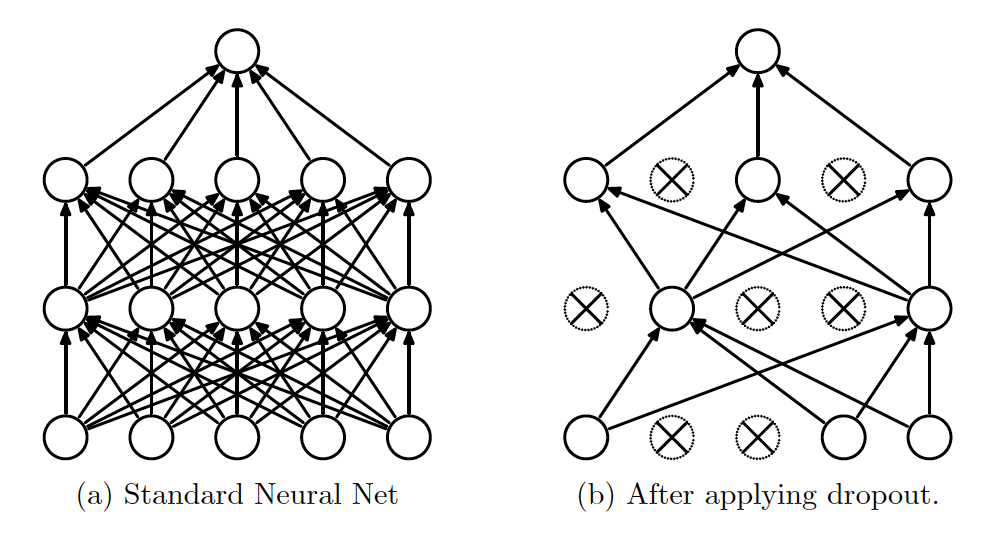
\includegraphics[scale=0.4]{hw5/dropout.png}
\end{center}
\end{figure}


\subsection{PyTorch}

Before you start, please checkout this useful \textcolor{blue}{link}\footnote{\url{https://pytorch.org/tutorials/beginner/deep_learning_60min_blitz.html}} that explains the basics of \textbf{PyTorch} library, so that you feel comfortable with its classes and methods.
\vspace{5mm}

We provided you with the \textit{data.py} file that creates the dataloaders for train and validation with 10,000 images each from the CIFAR dataset that you explored before.

\subsection{Instructions}
\begin{itemize}
\item Read \textbf{PyTorch}'s documentation and load the CIFAR data.
\item You will need to complete the missing code (marked with \#TODO) in the script provided, \textbf{\textit{dropout\_classifier.py}}.
\item Complete the function \textbf{\textit{\_initialize\_network}} method in \textit{dropout\_classifier.py} that defines the architecture of the neural network. The neural network must have 3 hidden layers (the number of neurons of each layer is specified in the hyper-parameters) with ReLU activations. You need to add dropout regularization after the input layer and after each hidden layer. (Hint: Use the nn.Linear(), nn.ReLU(), nn.Dropout() modules.)

\item Complete the \textbf{\textit{fit}} method. You need to add the forward pass (compute predictions), compute the cross entropy loss \footnote{see \url{https://pytorch.org/docs/stable/generated/torch.nn.CrossEntropyLoss.html}} and define the backward step. (Hint: use a linear layer for the output\_layer and cross entropy loss [note that in deep learning people refer to the logits as these final activations]).

\item Complete the \textbf{\textit{evaluate\_cross\_entropy}} method which computes the mean cross entropy loss for the full sets. (Hint: this function is analogous to the \textbf{evaluate\_accuracy} method.)


\item Train your classifiers, we provided you with beginning code in the \textbf{\textit{main}} function. (Hint: trajectories will be available in the \textbf{\textit{trajectories}} attribute of the classifier, save the weights of your classifiers so that your progress is not lost.)

\item You should be able to reach around 50\%
test accuracy with 0.5 dropout probability (notice this is a 10 class classification task). The original paper runs the optimization for a million steps, try to run your classifiers for at least \textbf{a hundred thousand steps} (refer to the initial instructions on how to train NNs using Google colab), keep in mind that you should be able to almost perfectly fit the training set (close to 100\% accuracy).

\end{itemize}

\subsection{Expected Results}
Finally, for the following values of dropout probability (parameter \textit{hidden\_dropout\_prob} in params list) $p\in\{0.0, 0.2, 0.5, 0.8\}$ report the following :
\begin{enumerate}[a]

    \item (10 points) Train your classifiers (using GPU) for \textbf{a hundred thousand steps}. You may run your algorithm for \textbf{ten thousand steps} (using CPU) and you will be awarded full points for the next results, but won't receive this 10 points.
    
    \item (25 points) In the same plot, display the train and val loss vs the gradient steps (only for the given display steps specified in the hyper-parameters, each display is expensive to compute).

    \item (25 points) Plot train and val accuracy vs gradient steps (only for the given display steps specified in the hyper-parameters).
    
    % \item (30 points) Plot the input\_layer's learnt filters (weights) of 25 units (of your selection), plot on a 5x5 grid figure. For this filters plot, the weights must be normalized to be between 0 and 1, using the min and max of all the weights. For this use the \textbf{\textit{get\_filters}} method.

    \item (20 points) Report the final loss and accuracy for train and val sets. Provide your comments on the relationship between generalization and regularization.
    
    \item (20 points) Please briefly explain why at the test time, the learned weights need to be scaled down by multiplying the probability of dropout (feel free to refer to the dropout paper to answer this question).
    
\end{enumerate}

\end{document}